% work in progress

\chapter{Expert Questionnaire}\label{chapter: expert}

	\section{Expert Selection}
	
	\section{Questionnaire}
	\subsection{Solutions Overview Draft}
	\subsection{Questions}

	\section{Results}
	
	
\chapter{Reference Implementation}\label{chapter: implementation}

This chapter focuses on the development of a reference implementation covering the \ac{vc} lifecycle, which is based on learnings of the last few chapters concerning theoretical background and expert opinions. It is intended to directly address the lack of practical considerations of \ac{SSI} solutions in the research area, by leveraging four of the previously listed solutions that can be used to implement the \ac{vc} lifecycle. In the next sections, the complete implementation process will be described, starting with preliminary considerations and ending with results and lessons learned.

    \section{Considerations}\label{section: ri-considerations}
    % Considerations: What should be done? Why? What's important? What not? Which implementations have i chosen? Which language for reference implementation? Why API?
    As previously stated, the reference implementation should exemplarily implement four solutions in such a way that they map, based on their capabilities, the \ac{vc} lifecycle as much as possible. This enables a practical validation of the promises made by the solution providers and can thus provide a thorough insight into the existing or missing range of functionality. This way, possible blind spots or even insufficient features can be identified, which can be used to further improve the available solutions. This approach can additionally generate added value for developers who want to use \ac{SSI} technologies in their projects, since actual experiences, capabilities, and code from a real implementation process can be reused.
    
    Since the results of the implementation are also to be incorporated directly into a new developer-oriented evaluation framework, there are some key considerations that must be defined beforehand. To meet the objectives described in this section, the following considerations were established:
    % Maybe add something along the lines of: MVP -> i don't care about error handling and edge cases
    \begin{itemize}
        \item \textit{Use-case agnostic}: In order to represent the \ac{vc} lifecycle as broadly and standardized as possible, the reference implementation should not be bound to the requirements and specifics of a use case. Focusing on a specific use-case could possibly lead to certain parts of the \ac{vc} lifecycle being underrepresented or not implemented at all. Such an open approach can also invite a closer look and implementation of specific facets of a technology that would have been unnecessary for a use case. This also means that the reference implementation must be accessible in such a way that it can be used relatively independently of the technology stack being used for a potential use case.
        \item \textit{Flexible architecture}: The reference implementation should leverage a software architecture that makes it straightforward to plug in different \ac{SSI} solutions. Peculiarities and complexities should be abstracted away to create a flexible and resilient architecture. 
        \item \textit{Community efforts}: Since the \ac{SSI} community is very active, it should be checked beforehand which previous work can be reused for the implementation. This applies to both the architecture and the software libraries used. In this way, it can be ensured that the work does not disregard the considerations and requirements of the community.
        \item \textit{Implementation experience}: Throughout the entire development process, objective experiences and findings should be documented and summarized. As already mentioned, these may be relevant for other developers, the solution providers, and also for the mentioned evaluation framework.
    \end{itemize}
    
    Taking these four points into account, the goal is to create a reference implementation that is helpful for developers and meaningful for the evaluation framework. The next section explores this, starting with the base implementation and community efforts to date, on which further work can be based on.
    
    \section{Base Implementation}\label{section: base-implementation}
    % Basis for Implementation: vc-http-api -> why? What is it for? What changes/ additions have to be made? Why can I hijack it? API Document!
    % Technical basis -> express app, typescript 
    A RESTful API was chosen as the basic implementation form, since it is technology-independent and can be used in various programming languages and environments. It is only necessary that HTTP requests can be sent, which allows a high degree of flexibility in later applications. 
    
    As a basis, this work is roughly based on the ideas of the W3C Credentials Community Group, which has created an unofficial draft API definition called “Verifiable Credentials HTTP API”. This describes the structure of an API with all its routes, request, as well as response bodies, which can be used for the \ac{vc} “lifecycle management”. The group defined API contracts according to the OpenAPI standard, which were originally intended to be used as a basis for verifying interoperability of \acp{vc} issued by different providers (see interoperability report from \cite{homeland_security_preventing_2020}). It is important to note that the reference implementation is based on the state of the API contract as of April 2020 (v0.0.2-unstable), as some small things have changed since then. The contract is strongly based on the \ac{vc} standard and divides the API into resources for the three roles issuer, verifier, and an optional holder. This includes resources for issuing and verifying \acp{vc}/ \acp{VP}, and deriving, as well as revoking \acp{vc}. At this point, it should be emphasized again that this is an API definition and not an actual implementation. \cite{world_wide_web_consortium_credentials_community_group_vc_2021, world_wide_web_consortium_credentials_community_group_verifiable_2021}
    
    With regard to the reference implementation, this preliminary work is quite helpful, even if it doesn't fully cover the whole \ac{vc} lifecycle. Therefore, some changes and additions have been made. A graphical representation of the API definition is shown in figure \ref{figure: api definition}, which also allows testing of the individual routes.
    \newpage
    \begin{figure}[ht]
        \centering
        \makebox[\textwidth]{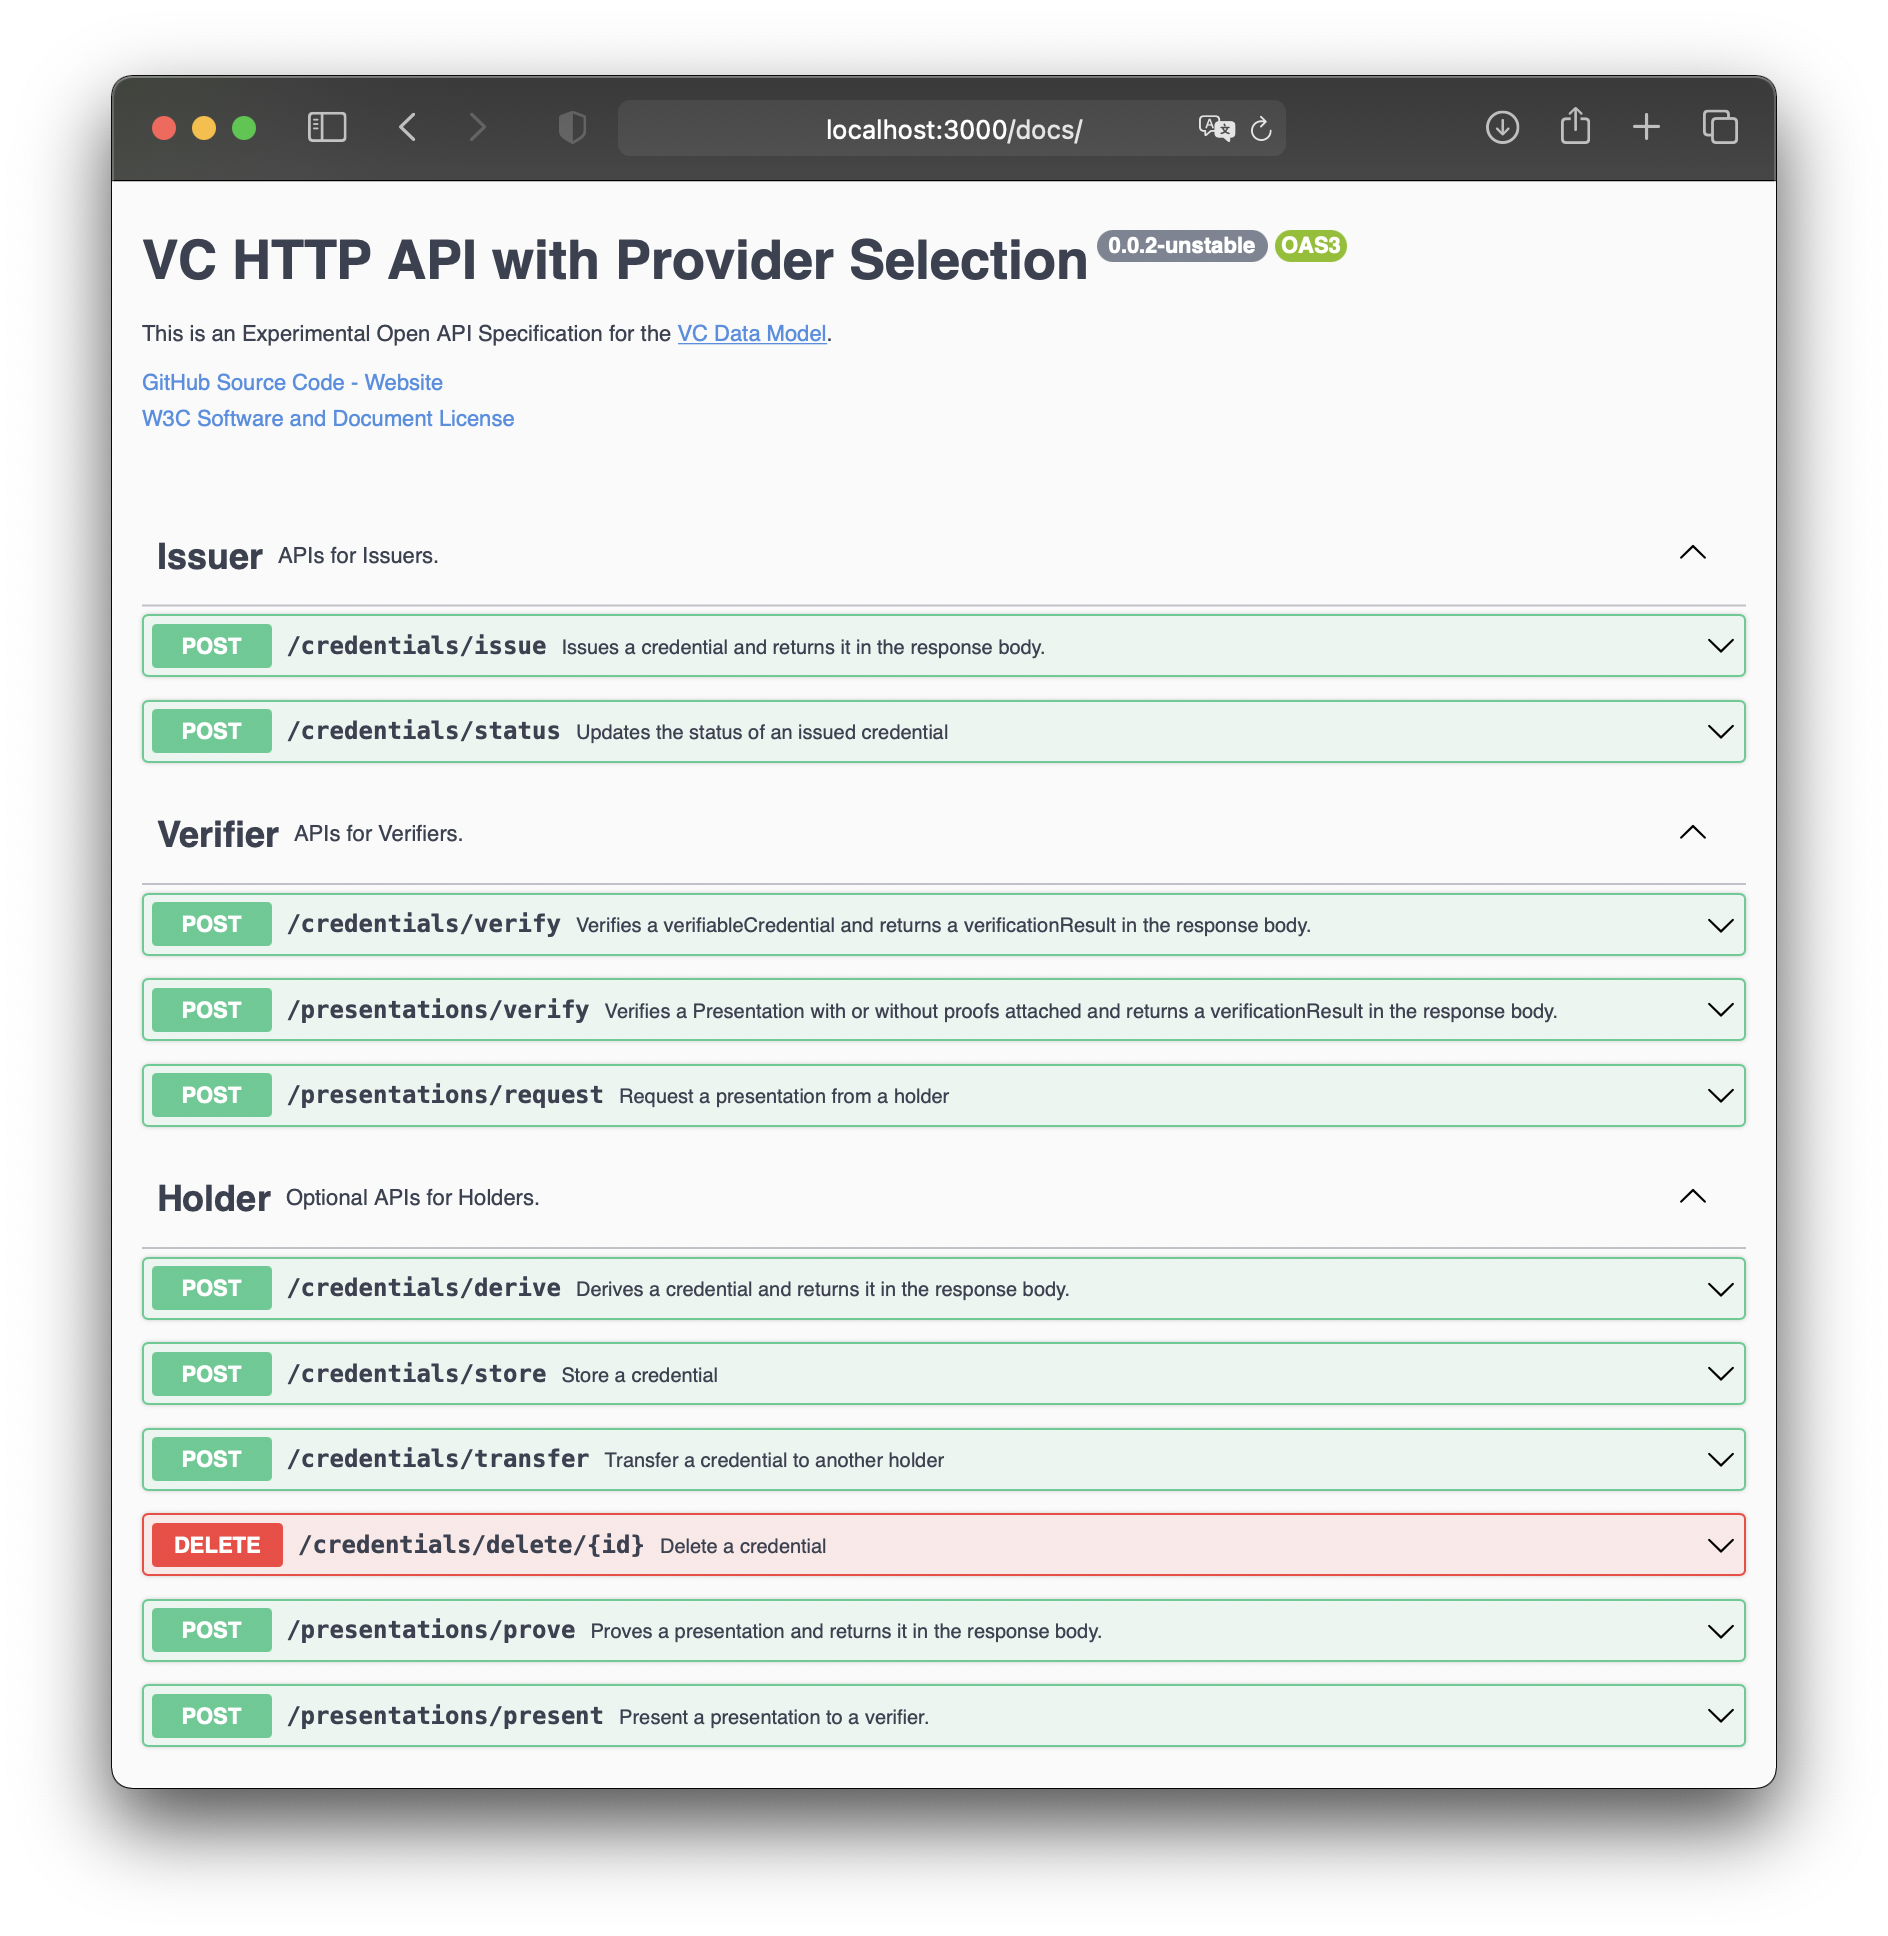
\includegraphics[width=0.9\textwidth]{thesis/img/13_api_definition.png}}
        \caption{Modified API definition (based on \cite{world_wide_web_consortium_credentials_community_group_vc_2021})}
        \label{figure: api definition}
    \end{figure}
    
    All changes made to the original definition are summarized by the following points:
    
    % TODO: might be incomplete 
    \begin{itemize}
        \item \textit{Provider selection}: Since four solutions should be addressable via the API, a query parameter was added to each route, which is based on a custom provider schema definition. Thus, it is possible to specify which solution/ provider should handle a request.
        \item \textit{Destination selection}: Another query parameter allows defining whether a request has the local or a remote agent as target. This mainly includes the issuing route for a \ac{vc}, which allows a \ac{vc} to be sent directly to the subject's agent via DIDcomm or QR code. In other cases, such as transferring \acp{vc} or presenting or requesting presentations, this can be done directly via the request body. For this purpose, the schema \texttt{GenericMessage} was defined, which in its structure is very roughly based on the DIDComm data model.
        \item \textit{Added routes}: To complete the lifecycle coverage, a route to create a presentation request has been added to the verifier, as well as routes to save, delete, transfer \acp{vc} and presenting \acp{VP} to the holder. For the request and response bodies, existing schemas were reused as much as possible.
        \item \textit{Response bodies}: Since some response bodies contained too many unnecessary attributes for the requirements of the API, the schema \texttt{GenericResult} was introduced, which only describes whether the operation was successful and whether there were errors. This schema is used for verifying, storing, deleting, and transferring \acp{vc} and verifying, as well as requesting/ presenting \acp{VP}.
    \end{itemize}
    
    The goal of the customizations was to ensure that the original API definition did not constrain the implementation, while retaining fundamental parts of the community work. 
    
    Based on the expert survey and observations from the IIW April 2021, the solutions Veramo from ConsenSys Software Inc., MATTR VII from MATTR Limited, Trinsic Core from Trinsic Technologies Inc., and Azure AD Verifiable Credentials from Microsoft were selected as the four solutions to be included in the reference implementation. For the implementation language, TypeScript was chosen as it was the only language where Veramo, Trinsic and Azure offer SDKs for. In addition, other basic libraries in the \ac{SSI} area are written in TypeScript or at least JavaScript and would thus integrate more easily into the implementation to possibly add missing features. Unlike JavaScript, various features of TypeScript allow cleaner and more robust code \cite[p. 87]{zammetti_modern_2020} that can simultaneously benefit from much of the existing JavaScript packages being made available from the open-source community. //move
    
    Building on this decision, node.js was selected as the JavaScript runtime that can be used in combination with the express.js library to develop highly scalable web applications such as APIs \cite{openjs_foundation_about_2021, openjs_foundation_express_2021}. To make TypeScript work in this environment, various dependencies such as TypeScript, ts-node, eslint, and some type definitions were installed via the Node Package Manager. The next section describes how these components and the four solutions were combined into a flexible software architecture.
    
    \section{Architecture}\label{section: architecture}
    % Software architecture, factory method pattern -> why? Describe how solutions tap into it.
    
    With regard to the considerations in section \ref{section: ri-considerations}, the factory method design pattern was chosen for the software architecture. It belongs to the creational patterns and thus influences how the instantiation process is carried out. A developer can thereby decide independently of the system how objects are created, which enables a high degree of flexibility. It defines an interface or an abstract class for the creation of objects, whereby the instantiation of objects is done by subclasses instead of a class. This is useful, for example, if a class does not yet know which objects it needs to create at runtime. \cite[pp. 81, 85, 107-108]{gamma_design_1995} 
    
    This is pattern is appropriate because a request determines which solution and thus which objects have to be created. In addition, it allows the complexities of the individual solutions to be abstracted away, so that when defining the individual routes, only the concrete factory class must be called, which returns the correct object of the requested solution. This way, the routes only need to be programmed once and additional solutions can be added afterwards without having to change the code of the routes. Figure \ref{figure: factory method} shows a UML diagram that represents the concrete factory method pattern in the reference implementation. The interface \texttt{Factory} defines a method \texttt{createProvider()}, which is implemented by the class \texttt{ServiceProviderFactory}. This is the class which is instantiated, for example, in the routes and which is used to retrieve the object of a provider. A provider is the class of one of the four solutions that implements basic methods like the \ac{vc} issuance defined by the \texttt{ServiceProvider} interface.
    
    \begin{figure}[ht]
	    \centering    	    \makebox[\textwidth]{\includesvg[inkscapelatex=false, width=0.8\textwidth]{img/14_uml_ref.svg}}
        \caption{Factory method pattern in reference implementation (extracted and edited from \cite[p. 107]{gamma_design_1995})}
        \label{figure: factory method}
    \end{figure}
    
    A second pattern, which was integrated, is the Singleton design pattern. This is used in the individual concrete provider classes and allows that only one globally callable instance of a provider class can be created \cite[p. 127]{gamma_design_1995}. The rationale for this is that no more than one object is needed, caching is simplified, and multiple provider objects could lead to unforeseen complications.
    
    Looking at the complete system architecture, the previously described software architecture integrates tightly. The service provider factory sits between the routes for issuer, verifier, and holder and the concrete classes of the individual providers. Its manifestations in the architecture can be summarized as follows and can be seen in figure \ref{figure: sys architecture}:
    
    \begin{itemize}
        \item \textit{Veramo Provider}: The provider class requires an agent class from Veramo, which enables the integration of extensions for various functionalities. This can be, for example, the Uniresolver for resolving \acp{DID} or various services with which a connection to blockchains can be established for various actions (e.g. Infura or Microsoft's anchoring service). The agent also offers a REST API, which allows any actions to be executed from a remote location. Furthermore, the agent can connect to other Veramo agents on the Internet and, for example, exchange messages of any kind via DIDComm or resolve their \acp{DID}. A more detailed explanation of Veramo can be found later in subsection \ref{subsection: veramo}.
        \item \textit{MATTR Provider}: This provider communicates directly with the MATTR API, which handles any operations. Additionally, there is a callback service between the API and the provider, which can receive verification results from the MATTR platform, e.g. triggered by scanning a QR code through a mobile wallet.
        \item \textit{Trinsic Provider}: Similar to the MATTR provider, this also communicates directly with the Trinsic API and a callback service catches verification results. Thus, as with MATTR, the actual \ac{SSI} logic is outside the reference implementation.
        \item \textit{Azure Provider}: This provider is integrated into the architecture similar to MATTR and Trinsic. 
    \end{itemize}
    
    \begin{figure}[ht]
        \centering
        \makebox[\textwidth]{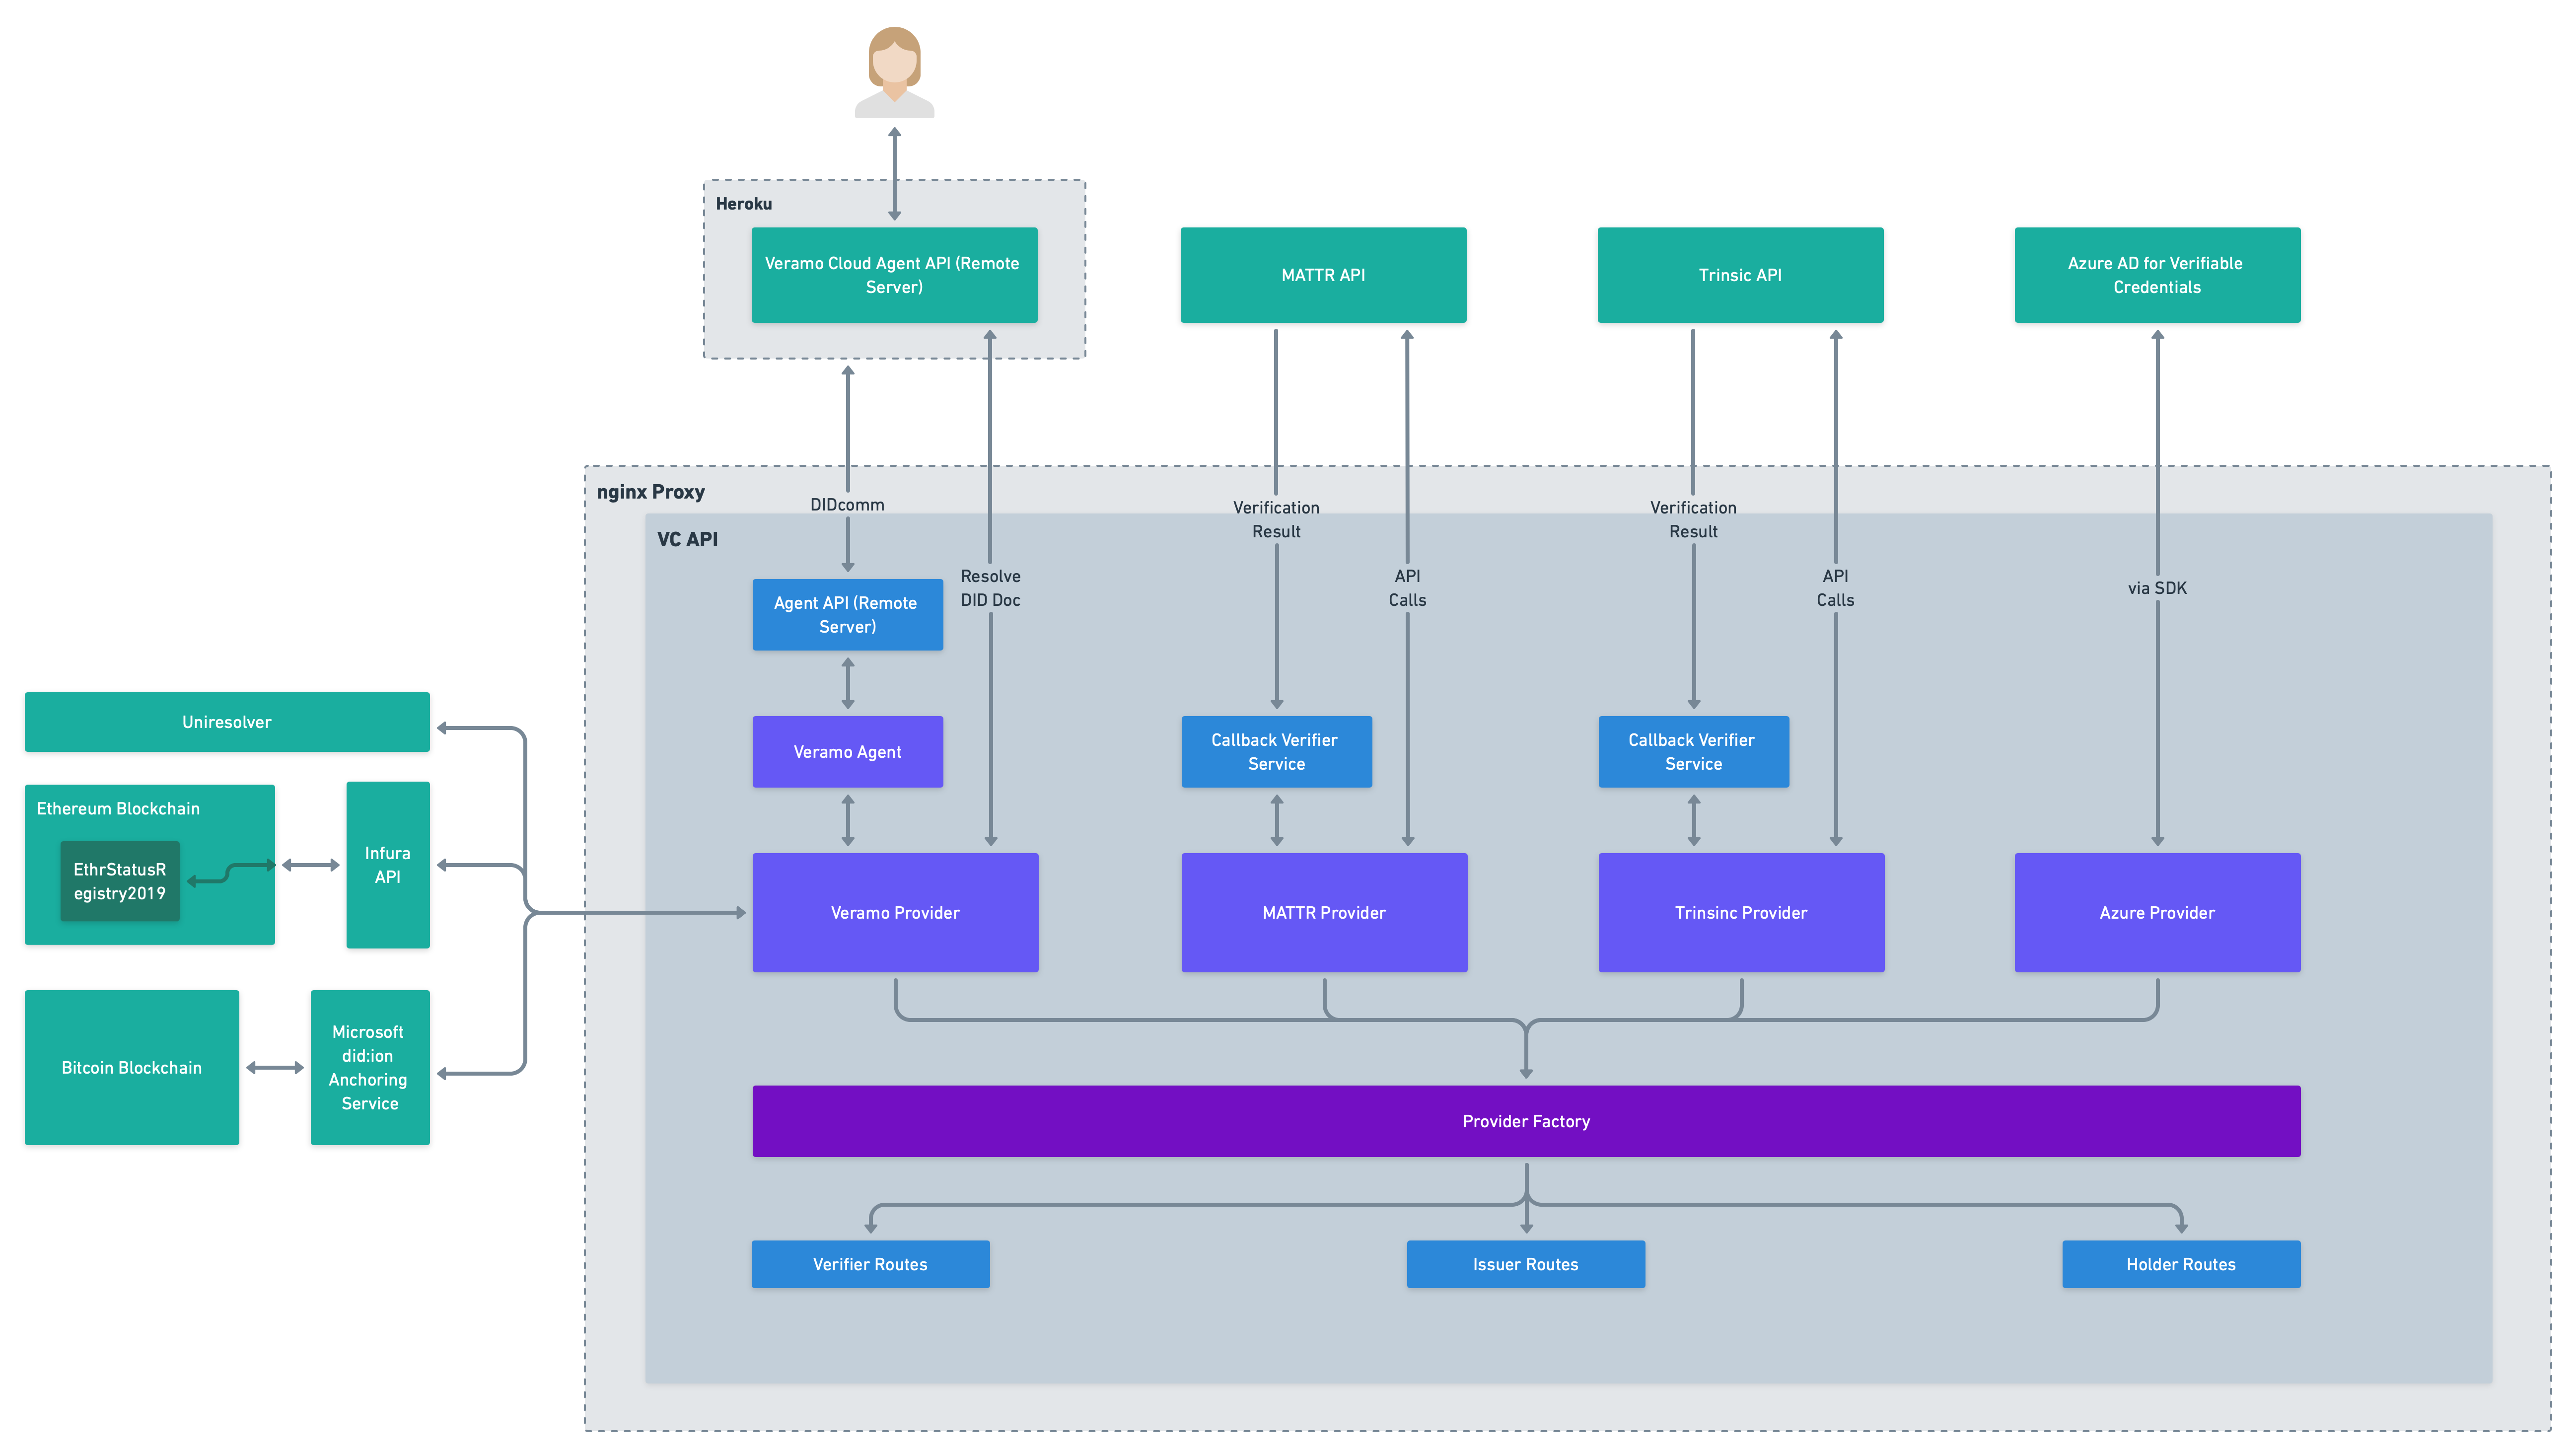
\includegraphics[width=\textwidth]{thesis/img/15_architecture.png}}
        \caption{System architecture}
        \label{figure: sys architecture}
    \end{figure}
    
    The addressed components form the reference implementation and are enclosed only by a nginx proxy. This proxy is assigned a domain so that external components can correctly address internal components such as callback or messaging services. 
    
    \section{Solution Integration}\label{section: integration}
    % Describe implementation process, what has been done, what not. What worked, what not? What was problematic? What did I like?
    
    This section briefly introduces each of the solutions and addresses their implementation. First, however, the concepts of the last section will be discussed with regard to their implementation. The goal is to establish a conceptual skeleton into which the following subsections can be seamlessly integrated.
    
    The starting point is \texttt{index.js}, which starts the web server and thus the API via Express by bundling all routes from other files here. These are divided into the files \texttt{HolderRoutes.ts}, \texttt{VerifierRoutes.ts}, and \texttt{IssuerRoutes.ts} and implement the associated methods. Listing \ref{listing: verifier routes} shows an example of a section of \texttt{VerifierRoutes.ts}.
    \newline

\begin{lstlisting}[style=ES6, caption=Extract of verifier routes, label={listing: verifier routes}]
const router = express.Router();
const factory = new ServiceProviderFactory();

router
  .post("/credentials/verify", providerCheck, async(req, res) => {
    const query = req.query.provider.toUpperCase();
    const body = req.body.verifiableCredential;
    
    const provider = factory.createProvider(ServiceType[query]);
    const result: GenericResult =
      await provider.verifyVerifiableCredential(body);
      
    if (result instanceof Error) {
      res.status(500).send(<GenericResult>{ 
        success: false, 
        error: result.message 
      });
    } else {
      res.status(200).send(result);
    }
  })
  ...
export = router;
\end{lstlisting}

    Here, the POST method for verifying a \ac{vc} is attached to the \texttt{router} (line 10). A \texttt{providerCheck} is appended as middleware, which checks whether the provider specified in the query is indeed valid. Within the route body, the provider object is created via the \texttt{ServiceProviderFactory}, which should handle the request (line 14). This object is then used in lines 15 and 16 to verify the \ac{vc} in the request body, the result of which is then sent as a response to the requestor. By exporting the router object (line 28), all injected routes can be imported into \texttt{index.js} and made available. This example shows that no provider-specific code is present in the route code due to the factory method pattern. To demonstrate how the \texttt{ServiceProviderFactory} works, its code can be seen in listing \ref{listing: factory}.
    \newpage
\begin{lstlisting}[style=ES6, caption=Extract of service provider factory, label={listing: factory}]
export class ServiceProviderFactory implements Factory {
  createProvider(type: ServiceType): ServiceProvider {
    switch (type) {
      case ServiceType.VERAMO:
        return VeramoProvider.getInstance();
      case ServiceType.MATTR:
        return MattrProvider.getInstance();
      case ServiceType.TRINSIC:
        return TrinsicProvider.getInstance();
      case ServiceType.AZURE:
        return AzureProvider.getInstance();
      default:
        return null;
    }
  }
}
\end{lstlisting}

    The class \texttt{ServiceProviderFactory} implements the \texttt{createProvider} method according to the \texttt{Factory} interface. If this method is called with the desired provider (ServiceType), as e.g. in listing \ref{listing: verifier routes} line 14, then the Singleton object corresponding to the provider is returned via a switch statement. According to the factory method pattern, all provider classes implement the \texttt{ServiceProvider} interface and its signatures as concrete methods. This can be seen exemplarily in listing \ref{listing: provider}.

\begin{lstlisting}[style=ES6, caption=Example of provider implementation, label={listing: provider}]
export interface ServiceProvider {
  deleteVerifiableCredential(identifier: string): 
   Promise<CredentialDeleteResult>;
  ...
}

export class VeramoProvider implements ServiceProvider {
  async deleteVerifiableCredential(identifier: string): 
   Promise<CredentialDeleteResult> {
    const db = new VeramoDatabase();
    const result: CredentialDeleteResult = { isDeleted: false };
    try {
      const isDeleted = await db.deleteCredential(identifier);
      result.isDeleted = isDeleted[0];
      result.message = isDeleted[1];
      return result;
    } catch (error) {
      return error;
    }
  }
  ...
}\end{lstlisting}

    In this case, the class \texttt{VeramoProvider} implements the interface \texttt{ServiceProvider} with its signatures like \texttt{deleteVerifiableCredential()} concretely, to delete a \ac{vc} from the Veramo agent database.
    
    Having described the programmatic skeleton, the following subsection describes the first solution MATTR and its integration into the reference implementation.
    
    \subsection{MATTR}\label{subsection: mattr}
    MATTR Limited is a New Zealand-based company \cite{mattr_privacy_2021} that specializes in providing solutions for “[...] a new world of digital trust.” \cite{mattr_mattr_2021-4}. This primarily includes their MATTR VII platform, which can be used to technically implement key components of an \ac{SSI} ecosystem \cite{mattr_products_2021}. According to the company, the platform can be divided into the following components: \cite{mattr_mattr_2021-2}

    \begin{itemize}
        \item \textit{VII Core}: Since MATTR is a platform solution, Core includes a variety of web APIs that serve as the foundation. This includes APIs for \acp{DID}, \acp{vc}, \acp{VP}, and secure messaging between \acp{DID}. \cite{mattr_vii_2021}
        \item \textit{VII Extensions}: These are additional components that build on VII Core, such as a bridge for OpenID Connect systems (see user-centric identities), or white label mobile wallets and SDKs. \cite{mattr_vii_2021-1}
        \item \textit{VII Drivers}: Similar to PCs, this component allows flexible integration of basic elements. This includes support for various DID methods (did:key, did:web, did:sov), crypto suites (ed25519, bls12381g2)\cite{mattr_vii_2021-2}, and storage options. \cite{mattr_vii_2021-3}
    \end{itemize}
    
    In addition, the company offers resources for developers to learn the basics of SSI \cite{mattr_resources_2021} but also a comprehensive API documentation, tutorials in written and in some cases video form \cite{mattr_mattr_2021}, mobile wallets, and sample app \cite{mattr_mattr_2021-1, mattr_vii_2021}. Within the \ac{SSI} community, they participate in the development of open standards \cite{mattr_approach_2021, looker_bbs_2021} and software libraries \cite{mattr_mattr_2021-5} and have demonstrated interoperability  in the Homeland Security Plugfest in 2021 \cite{homeland_security_interoperability_2021}.
    
    With regard to the integration into the reference implementation, the generous free tier and the  well-structured documentation proved to be very helpful. Thus, a large part of the \ac{vc} lifecycle could be integrated relatively unproblematically by simply addressing the corresponding endpoints of the MATTR VII REST API. These take care of any logic and can also be used to manage \acp{DID} and their keys as well as \acp{vc}. The support of BBS+ for ZKP credentials, revocable credentials (RevocationList2020) and LD proofs is directly integrated into the API as well. For interactions like issuance and presentation with the MATTR mobile wallet, an OIDC provider (see user-centric identity) like Auth0 is currently necessary. Its initial setup took some time, but was feasible due to the good documentation. To receive the verification result from a mobile wallet presentation, the sample apps were used to integrate a callback service into the reference implementation. In summary, the broad coverage of the \ac{vc} lifecycle, the large number of features, and the very developer-friendly documentation with tutorials stood out positively.
    
    Nevertheless, some things were noticed that could be problematic and restrictive under certain Partialumstances. For example, on-boarding to the platform has been relatively cumbersome in April 2021, as it was necessary to join the official Slack channel after successful registration, where support then triggers the rest of the process manually. After the cloud agent had been created, the password was communicated by the support via Keybase. Additionally, some features are not or only partially usable in combination, such as the support of BBS+ only for credentials based on did:key. Support for additional DID methods based on public permissionless distributed ledgers such as did:ion would also be desirable, which, unlike did:key, can also include other metadata such as messaging endpoints. In addition, an SSI native implementation for interactions with mobile wallets is missing, which could theoretically take place via DIDComm. This complicates things, since the MATTR platform requires an OIDC issuer and templates for e.g. presentations to be created for each type of credential that is to be issued to a mobile wallet. However, MATTR is already working on a \ac{SSI} native solution [citation needed]. The use of the OIDC provider is also limiting, as the only way to map the OIDC attributes to the JSON-LD attributes is to use the schema.org vocabulary. Custom schemas are not supported. Finally, it should be noted that the private keys for all \acp{DID} are managed by MATTR and cannot be exported by users. None of the mentioned problems can be solved by the developer through individual implementations, which seems to be an inherent problem of the platform infrastructure, which can only be managed by MATTR.
    
    The majority of the integration took place in \texttt{MattrProvider.ts}, which implements the \texttt{ServiceProvider} interface. Since this class implements any functionality via HTTP requests, listing \ref{listing: mattr verification} is an example of how this works. However, it should be noted that methods such as \texttt{issueVerifiableCredential()} are significantly more complex, as specific logic such as the distinction in issuance to a wallet or not must be considered accordingly.
    \newline
    
\begin{lstlisting}[style=ES6, caption=Example of mattr verification implementation, label={listing: mattr verification}]
async verifyVerifiablePresentation(body: VerifiablePresentation): 
 Promise<GenericResult> {
  const request = { presentation: body };
  const authToken: string = await this.getBearerToken();
  const result: GenericResult = {
   success: null,
  };

  try {
    const response = await fetch(`.../presentations/verify`, {
      method: "POST",
      body: JSON.stringify(request),
      headers: { 
        "Content-Type": "application/json", 
        Authorization: `Bearer ${authToken}` 
      },
    });
    const verificationResult = await response.json();
    result.success = verificationResult.verified;
    result.error = verificationResult.reason;
    return result;
  } catch (error) {
    return error;
  }
}\end{lstlisting}
    
    Furthermore, helper methods were implemented to generate authentication tokens for the requests or to cache QR codes for issuing \acp{vc} to mobile wallets. Especially, interactions with the latter required several extra implementations that enable the generation of issuance and presentation requests in the form of QR codes via an OIDC provider to MATTR. Starting with the issuance of a \ac{vc} to such a wallet, the type, and attributes of the \ac{vc} must be prepared at the OIDC provider and MATTR. The resulting provider ID can then simply be referenced in an issuance URL and, if desired, encoded in a QR code. By scanning this, the associated VC can be obtained directly in the MATTR wallet app. This code is part of the \texttt{MattrVerifierService.ts} and can be seen in listing \ref{listing: mattr oidc issuance}.
    \newline
    
\begin{lstlisting}[style=ES6, caption=OIDC issuance QR code generation, label={listing: mattr oidc issuance}]
private getOIDCIssuerQRCode(oidcIssuer: string): Buffer {
  if (this.issuerQrCache.has(oidcIssuer)) 
    return this.issuerQrCache.get(oidcIssuer).image;

  const qrcode: Buffer = qr.imageSync(
    `openid://discovery?issuer=${process.env.MATTR_URL}
    /ext/oidc/v1/issuers/${oidcIssuer}`,
    { type: "png" }
    );
  this.issuerQrCache.set(oidcIssuer, qrcode);
  return qrcode;
  }
}\end{lstlisting}

    To verify a \ac{vc} from the MATTR wallet app, a presentation request must be prepared. For this purpose, a presentation template is first defined on the MATTR platform, which contains, for example, the allowed issuers or the requested attributes of a requested \ac{vc}. MATTR assigns a unique ID to this template. This ID can then be used in the first step of provisioning in the reference implementation. Here the actual presentation request is prepared with the verifier DID, the template ID, an expiration date and a callback URL via the MATTR API. In the next step, authentication keys are retrieved as a DID URL from the verifier DID document via the MATTR platform to sign the presentation request via the same platform in the next step. The resulting JWS payload is cached and a QR code is generated with a public URL of the reference implementation. This process can be seen in listing \ref{listing: mattr oidc presentation}.
    \newline
\begin{lstlisting}[style=ES6, caption=Generate QR code for OIDC presentation reqest, label={listing: mattr oidc presentation}]
public async generateQRCode(request: GenericMessage): Promise<Buffer> {
  const templateId: string = request.body.request.credentialType;
  
  // Check cache
  if (this.qrCache.has(templateId)) 
    return this.qrCache.get(templateId).image;

  // Prepare QR code and JWS payload URL
  const publicUrl = this.publicUrl;
  const provisionRequest = 
    await this.provisionPresentationRequest(publicUrl, request);
  const didUrl = await this.getVerifierDIDUrl(request.from)
  const didcommUrl = 
    await this.signPayload(publicUrl, didUrl, provisionRequest); 
  const qrcode = qr.imageSync(didcommUrl, { type: "png" });
    
  // Cache and return it
  this.qrCache.set(templateId, qrcode, request.expiresTime);
  return qrcode;
}\end{lstlisting}
    
    When the QR code is scanned with the MATTR wallet app, the qr route of the reference implementation is called, which returns the stored JWS payload url. This is the starting point for all further interactions between the wallet app and the MATTR platform. The callback route in the reference implementation allows MATTR to report whether the presentation was successful and the \ac{vc} could be verified. Both routes were defined via the express router.
    
    This describes the fundamental aspects of the MATTR implementation. In the next subsection, Trinsic will be discussed in the same context.
    \vfill
    
    \subsection{Trinsic}\label{subsection: trinsic}
    The Trinsic SSI platform is developed by the US company Trinsic Technologies Inc. and offers various components for developing SSI solutions \cite{trinsic_trinsic_2021}. The company divides the platform into four components:
    
    \begin{itemize}
        \item \textit{Trinsic Core}: Since Trinsic is also a platform solution, Core offers a lot of APIs to issue, verify and exchange credentials. \cite{trinsic_trinsic_2021-1}
        \item \textit{Trinsic Ecosystems}: Enables the creation of ecosystems based on organizations. It can be determined which credentials can be exchanged, who can participate in the ecosystem, and how participants can know who to trust. \cite{trinsic_trinsic_2021-2}
        \item \textit{Trinsic Studio}: A dashboard that builds a user-friendly GUI on top of the Core APIs to manage organizations, connections, credentials, and verification templates. Trinsic also offers a white-label version of Trinsic Studio. \cite{trinsic_trinsic_2021-3}
        \item \textit{Identity Wallets}: The wallet SDK allows the creation of cross-platform wallet apps for, for example, Flutter and React Native. Otherwise, Trinsic's own wallet app for Android and iOS can be downloaded from the app stores. \cite{trinsic_identity_2021}
    \end{itemize}
    
    In addition, Trinsic offers SDKs in various languages that serve as wrappers for the REST API, providing native interfaces for programming languages \cite{trinsic_service_2021}. This includes languages such as Ruby, Python, JavaScript and more, with SDKs for additional languages that can be generated via Trinsic's swagger hub. Also worth mentioning is the clearly structured and comprehensive documentation, which also integrates code samples and a getting started tutorial \cite{trinsic_introduction_2021}. The documentation also describes the basics of SSI in a short and concise way, so that even new developers can get an introduction to the topic. The registration process is very short and in combination with the free tier, which allows 50 credentials exchanges per month and has a reduced feature set \cite{trinsic_pricing_2021}, it is possible to get started quickly. The company is also partnered with Zapier, which allows custom flows to be created with other apps, e.g. to send a credential via Gmail when there is a new attendee at Eventbrite. Trinsic follows standards like \ac{DID}, \ac{vc}, DIDComm and various Aries RFCs, for which open-source work has been done on a .NET implementation \cite{trinsic_open_2021}.
    
    The integration of Trinsic into the reference implementation proved to be extremely pleasant. This was mainly due to the documentation but also to Trinsic Studio. With the latter, an organization and associated credential and verification templates could be created within a few minutes. The resulting IDs could later be used to trigger the issuance and presentation flows using Trinsic's JavaScript SDK, which also includes type definitions for TypeScript. No other solution made the implementation process so quick and easy.
    
    The Hyperledger focus is, however, very noticeable from a technological point of view. Only JSON credentials and CL signatures for revocation, DIDComm v1, Aries exchange protocols and Hyperledger-specific DID methods like did:sov are supported. Newer technologies as well as DID methods based on public permissionless blockchains would be appreciated here. In addition, functionality is abstracted away even further in contrast to MATTR, which increases user-friendliness but hardly allows any flexibility. Thus, no custom \acp{DID} can be generated, and no custom \acp{vc} can be issued or verified without first generating a template. Direct access for generating \acp{VP} on the cloud agent or the selective disclosure functions is also not available. All these things are managed in the background by Trinsic and the mobile wallet. This can certainly be sufficient for certain use cases, but maybe too inflexible for others. Just like MATTR, developers are completely dependent on Trinsic in terms of the tech stack and private key management. The company is trying to address many of the points mentioned above with the Core v2 platform, which is currently in closed beta. Latest technologies such as JSON-LD credentials, BBS+, presentation exchange, DIDComm v2 and new DID methods such as did:key or did:web are supported here. Trinsic could thus catch up with MATTR in terms of supported technologies. Table \ref{tab: trinsic roadmap} shows the current roadmap of the Trinsic platform.
    
        	\begin{center}
            \captionof{table}{Trinsic Roadmap (based on \cite{riley_hughes_announcing_2021})}
        		\begin{threeparttable}
            		\begin{tabular}{llll}
            			\hline 
            			Type & Current & Beta & Future\tabularnewline
            			\hline 
            			\textbf{Data Exchange} & JSON & JSON-LD   & JWT \tabularnewline
            			\textbf{}              & CL signatures    & BBS+ signatures       & OIDC SIOP\tabularnewline
            			\textbf{}              & Aries exchange   & Presentation exchange & \tabularnewline
            			\textbf{Communication} & did:peer         & did:key               & WACI\tabularnewline
            			\textbf{}              & DIDComm v1       & DIDComm v2            & BLE, NFC\tabularnewline
            			\textbf{}              & HTTP transport   & gRPC transport        & \tabularnewline
            			\textbf{Public Trust}  & did:sov          & did:key, did:web      & did:un, did:ion\tabularnewline
            			\textbf{}              & Hyperledger Indy & did:indy              & \tabularnewline
            			\hline 
            		\end{tabular}
        	\end{threeparttable}
        	\label{tab: trinsic roadmap}
    	\end{center}
    	
    The main part of the implementation takes place in the \texttt{TrinsicProvider.ts}, which implements the \texttt{ServiceProvider} interface. To communicate with the Trinsic API, the JavaScript SDK was used to create an object of the \texttt{CredentialsServiceClient} class. This is done in the constructor so that the object is available immediately after initialization. This can be seen in listing \ref{listing: trinsic service client}.
    \newline
    \begin{lstlisting}[style=ES6, caption=Connecting to Trinsic API via SDK, label={listing: trinsic service client}]
export class TrinsicProvider implements ServiceProvider {
  client: CredentialsServiceClient;

  private constructor() {
    this.client = new CredentialsServiceClient(
      new Credentials(process.env.TRINSIC_KEY), 
      { noRetryPolicy: true }
    );
  }
  ...
}\end{lstlisting}
    
    How to programmatically issue a \ac{vc} to the mobile wallet via Trinsic, for example, can be seen in listing \ref{listing: trinsic issuance}. As required by the \texttt{ServiceProvider} interface, this is done by implementing the \texttt{issueVerifiableCredential()} method that first checks whether the requester actually wants to issue a pre-defined credential to the wallet. If this is not the case, it is informed that only predefined credentials can be issued to a wallet. If everything is correctly defined, the ID of the credential template as well as the values for the attributes of the credential are obtained from the request body. The \texttt{GenericMessage} schema in the request body is used for this. An object is formed from these values, which is submitted to the API via the Trinsic SDK and results in a \texttt{CreateCredentialResponse} object. The \texttt{offerUrl} contained therein is then encoded in a QR code, which can then be scanned via the Trinsic wallet to retrieve the \ac{vc}. 
    \newline
    
    \begin{lstlisting}[style=ES6, caption=\ac{vc} issuance with Trinsic, label={listing: trinsic issuance}]
async issueVerifiableCredential(
  body: IssueCredentialRequest | GenericMessage,
  toWallet: boolean
): Promise<IssueCredentialResponse | Buffer> {
  try {
    if (!toWallet) throw Error("Only issuance to Trinsic wallet...");
    if (isGenericMessage(body)) {
      // Prepare request body for Trinsic
      const message: GenericMessage = body;
      const request = {
        definitionId: message.body.credentialType,
          connectionId: null,
          automaticIssuance: false,
          credentialValues: message.body.claimValues,
      };
      
      // Generate QR code with offer URL
      const vcOffer: CreateCredentialResponse = 
        await this.client.createCredential(request);
      const qrcode: Buffer = 
        qr.imageSync(vcOffer.offerUrl, { type: "png" });
      return qrcode;
    } else {
      throw Error("Issuing manual VCs is not supported...");
    }
  } catch (error) {
    return error;
  }
}\end{lstlisting}

    In the case of Trinsic, 3 of 10 methods of the \texttt{ServiceProvider} interface could be implemented directly, while all parts except for the transfer of \acp{vc} are at least indirectly part of Trinsic. Among them are the methods for issuing, deleting and creating presentation requests. The method for revoking credentials could have been implemented theoretically, but was not part of the free tier. After a presentation request has been successfully performed by the user, the result of the verification can be received via a webhook in the reference implementation. Similar to MATTR, a route was created via Express, to which the Trinsic platform can send the result. This webhook URL also had to be added via the Trinsic Studio beforehand, since the URL is not part of the presentation request body, as opposed to MATTR. Listing \ref{listing: trinsic webhook} shows how the webhook route is implemented.
    \newline
    
    \begin{lstlisting}[style=ES6, caption=Trinsic webhook for verification result, label={listing: trinsic webhook}]
const router = express.Router();
const trinsic = TrinsicProvider.getInstance();

router.post("/webhook", async (req, res) => {
  try {
    if (req.body.message_type === "verification") {
      const verification = 
        await trinsic.client.getVerification(req.body.object_id);
      console.log(verification);
    }
  } catch (error) {
    console.log(error.message || error.toString());
  }
  res.status(200).end();
});

export = router;
\end{lstlisting}

    At this point, all the specifics of the Trinsic platform and its integration into the reference implementation have been addressed. In the next subsection, the first and only non-platform solution and its implementation will be presented.
    
    \subsection{Veramo}\label{subsection: veramo}
    
    Unlike the previous solutions, Veramo is a JavaScript framework for Verifiable Data in the SSI context \cite{veramo_veramo_2021-1}. It is the direct successor to the uPort project \cite{uport_uport_2021}, which was started by ConsenSys in 2015 and discontinued in 2021 due to a changing SSI ecosystem and foundational issues. The work on Veramo started around 2020 under the name “DID Agent Framework” and was intended to learn from lessons learned from uPort by creating a modular architecture whose functionalities could be extended by plugins and used both on the web, mobile, and backend. \cite{uport_veramo_2021}
    
    Veramo is currently in public beta and is working with the W3C and the DIF \cite{veramo_veramo_2021-1}. The center of the framework is the Veramo Agent written in TypeScript, which enables the plugin architecture and exposes its functionality to the developer through a common interface. At all times the \ac{vc} and \ac{DID} standards are taken into account, while allowing complete freedom and flexibility in all other areas. The Veramo agent implements four basic components for messaging, identifiers, credentials, and keys, which can be seen in figure \ref{figure: veramo agent}. \cite{veramo_veramo_2021-2}
    
    \begin{figure}[ht]
	    \centering    	    \makebox[\textwidth]{\includesvg[inkscapelatex=false, width=\textwidth]{img/16_veramo_agent.svg}}
        \caption{Veramo Agent (extracted from \cite{veramo_veramo_2021-2})}
        \label{figure: veramo agent}
    \end{figure}
    
    The framework provides various core plugins, which generally allow things like creating and resolving \acp{DID}, as well as issuing, retrieving, and exchanging credentials \cite{veramo_veramo_2021-2}, while providing a template for creating custom plugins \cite{veramo_uport-projectveramo-plugin_2021}. Similar to MATTR and Trinsic, Veramo provides some posts on fundamentals on \acp{vc} and \acp{DID} and some quick guides with sample code on how to use Veramo regarding setup with Node, React, React Native, the CLI, and deployment options of the agent for Heroku and AWS \cite{veramo_veramo_2021-2}.
    
    The integration process of Veramo into the reference implementation proved to be a mixed experience. Especially the CLI offered a good first start to try out Veramo. Thus, all basic features like creating \acp{DID} and issuing and verifying \acp{vc} could be tested in advance without any implementation process. Within the implementation, the very high degree of flexibility was especially noticeable. None of the previous solutions supports so many DID methods (did:key, did:web, did:ethr, did:ion), whereas the connection to the Uniresolver allows resolving almost any DID. In terms of deployment options, the Veramo agent can be used in web frontends, smartphone apps, and backend systems through the TypeScript backend, while the agent's modularity also allows tasks to be distributed among different agents. This allows for different architectures where, for example, one Veramo cloud agent implements only key management, another implements the issuing of \acp{vc}, and the agent in the mobile wallet implements only messaging and credentials storage. Since the Veramo agent also exposes all of its functionalities via a REST API with OpenAPI documentation, similar to MATTR and Trinsic, all functions can also be used on non-supported platforms via HTTP requests. This is not possible with any of the other solutions. In addition, with the DIDComm v1 implementation, complex communications between Veramo agents could also be implemented, such as the transfer of credentials between holders. Because of the open access to these modules, pretty much any use case can be realized, which is not possible due to limitations in the other solutions. In the meantime, Veramo already offers a DIDComm v2 implementation \cite{veramo_blog_2021}. Especially for such messaging cases, it was very helpful that a Veramo agent could be created on Heroku with a one-click button, making such multi-agent flows testable. In addition, the React Native integration was tested, with which a demo mobile wallet could be created within a very short time, with which a user could manage and receive \acp{vc}. This is relevant because Veramo does not currently provide its own wallet app in the app stores. In contrast to the platform solutions, the flexibility but also the complete control over architecture, code, and data such as the \acp{vc} and the private keys of \acp{DID} stand out. Veramo and all its components are completely open-source, with the development team being quite active with commits and answering Q\&A as well as bug tickets on GitHub.  
    
    Nevertheless, there were a few things that complicated the implementation process. The now updated documentation was either outdated or not available at all in April 2021. Only the code of the CLI implementation could be used as a guide, which in combination with some guesswork and trial and error led to the desired goal. Even today, not all areas and features are covered so far, such as code and explanations for the messaging system, how to issue and verify credentials, how to resolve \acp{DID}, that there is a did:ion plugin, types of events in the event system and much more. The documentation really only covers the most necessary areas to get started, which may discourage some developers. Furthermore, there are some technological limitations, which are briefly listed below:
    
\begin{itemize}
    \item \textit{Credential type}: Currently only JWT credentials are supported. Support for JSON-LD signatures is currently being worked on [github citation needed].
    \item \textit{Revocation}: There are no official, up-to-date plugins for revocation. There is only a library from two years ago that can be used with manual effort in Veramo to create revocable credentials with did:ethr and later revoke them as well. Support for RevocationList2020 does not exist, but can be retrofitted with open libraries from digital bazaar due to Veramo's open architecture.
    \item \textit{Selective Disclosures \& ZKP}: Due to the nature of JWT credentials, this is not currently possible. Veramo recommends keeping credentials as atomic as possible so that the user can present individual credentials with only a few attributes. However, support for BBS+ in combination with LD proofs is planned.
    \item \textit{Verification}: There is no proper API for verifying \acp{vc} and \acp{VP}. Meanwhile, only the validity of the JWT can be checked, but it does not retrieve the \ac{DID} document for the issuer's public key, does not check for revocation, integrity, or other important parameters. The developer currently has to check all of these by itself. However, this is also being looked at by the development team, which is working on a comprehensive verification API.
\end{itemize}

    This makes it clear that Veramo is really a beta and that various areas are not yet ready. Nevertheless, it should be noted that, in contrast to the other solutions, the open architecture means that missing functions can be retrofitted at any time. This behaviour is also supported by the Veramo developers, as they want an ecosystem of community plugins.
    
    Looking at the reference implementation, there is more effort here compared to the platform solutions, as now any logic has to be implemented via the Veramo API itself. In the middle of this is the \texttt{VeramoProvider.ts}, which implements the \texttt{ServiceProvider} interface and thus all lifecycle-specific methods. In order to access the methods of the Veramo API and its included plugins, an object of the Veramo agent is created and exported in the \texttt{VeramoSetup.ts} so that it can be directly imported and used in various places. To create the agent, all necessary plugins must be imported in the form of libraries and taken into account when initializing the object. This can be seen exemplary in listing \ref{listing: veramo agent}. 
    \newline
    \begin{lstlisting}[style=ES6, caption=Veramo agent creation, label={listing: veramo agent}]
// Core interfaces
import { createAgent, IDIDManager, ... } from "@veramo/core";

// Core identity manager plugin
import { DIDManager } from "@veramo/did-manager";

// Credential Issuer
import { CredentialIssuer, ICredentialIssuer } from "@veramo/credential-w3c";

...

export const veramoAgent = createAgent<
  IDIDManager & IKeyManager & IDataStore & IResolver & ... >({
  plugins: [
    ...
    new KeyManager({
      store: new KeyStore(dbConnection, new SecretBox(secretKey)),
      kms: {
        local: new KeyManagementSystem(),
      },
    }),
    new DIDManager({
      store: new DIDStore(dbConnection),
      defaultProvider: "did:key",
      providers: {
        "did:key": new KeyDIDProvider({
          defaultKms: "local",
        }),
        ...
      },
    }),
    new DIDResolverPlugin({
      resolver: new Resolver({
        ...
        key: getDidKeyResolver().key,
        ...getUniversalResolverFor(["io", "elem", "sov"]),
      }),
    }),
    new CredentialIssuer(),
    new MessageHandler({ ... }),
    ...
  ],
});\end{lstlisting}
    
    This is only a small excerpt, but it demonstrates the rough concept and functionality. For the reference implementation, various plugins were implemented for storing and managing keys, \acp{DID}, \acp{vc}, \acp{VP} as well as messages, message handlers (DIDComm, JWT, ...), DID provider, DID resolver and credential issuance. In addition, event listeners were utilized to document verification results and submitted presentation requests. Especially the latter was helpful in testing the multi-agent messaging flows to let a cloud agent automatically respond to submitted presentation requests via its API. This part is relatively well documented, but there were problems implementing the message handlers correctly, which resulted in errors with the validation of messages like JWT credentials or DIDComm messages. The author's issue report on GitHub was answered by the Veramo developers on the same day. It was described that the order in which the different message handlers are integrated in the setup is significant and was incorrect in the reference implementation. Such small details are unfortunately not documented and cost considerable time to debug. That being said, the author was able to identify an actual bug during implementation where mismatches of signatures between a \ac{vc} and its \ac{VP} occur under certain Partialumstances. This report was also being responded to on the same day and a fix was rolled out in under two weeks. The developers appear to respond quickly and helpfully in general on GitHub [github issues citation].
    
    With regard to the actual implementation of the lifecycle in the \texttt{VeramoProvider} class, the methods of the Veramo agent proved to be well usable. Basic methods for creating \acp{vc}, \acp{VP}, verifying messages like JWT credentials and sending presentation requests are provided, the latter being called Selective Disclosure Requests by Veramo. Looking at the descriptions of this topic in subsection \ref{subsection: bbs} and the nature of JWT credentials, the term selective disclosure is not well-chosen, since only a set of credentials and not a set of attributes of one credential are disclosed here. In listing \ref{listing: veramo issuance} is a code snippet for creating a \ac{vc} using the Veramo agent.
    \newline
        \begin{lstlisting}[style=ES6, caption=Issue a \ac{vc} with Veramo, label={listing: veramo issuance}]
async issueVerifiableCredential(body: IssueCredentialRequest, 
 toWallet: boolean): Promise<IssueCredentialResponse> {
    try {
      body.credential.issuer = { id: body.credential.issuer.toString() };
      const save: boolean = body.options.save ? body.options.save : false;
      const credential: W3CCredential = body.credential;
      
      const verifiableCredential: W3CCredential = 
       await veramoAgent.createVerifiableCredential({
        save: false,
        credential,
        proofFormat: "jwt",
      });

      // Prepare response
      const result: IssueCredentialResponse = {
        credential: verifiableCredential,
      };

      if (toWallet) {
        try {  // Send VC to another Veramo agent
          const msg = await veramoAgent.sendMessageDIDCommAlpha1({
            save: true,
            data: {
              from: verifiableCredential.issuer.id,
              to: verifiableCredential.credentialSubject.id,
              type: "jwt",
              body: verifiableCredential.proof.jwt,
            },
          });
          result.sent = true;
          return result;
        } catch (error) {
          return error;
        }
      }
      return result;
    } catch (error) {
      return error;
    }
  };\end{lstlisting}
    
    At the beginning, the credential object is prepared, which is then converted to an \ac{vc} in lines 8 to 13 using the methods After that, the API response is prepared with the created \ac{vc}, or if an error occurs during issuance, the error is sent directly to the requester as a response. If the request to the API defined that the \ac{vc} should be sent directly to the agent of the DID via the messaging endpoint, lines 21 to 35 handle this, using the \texttt{sendMessageDIDCommAlpha1()} method. This method has been deprecated and should be replaced by the new DIDComm v2 implementation. Considering the scope of this work, a short-term implementation of the new module has been omitted at this point. This feature is useful, for example, to send a \ac{vc} directly to the Veramo agent of a mobile wallet. MATTR and Trinsic offer similar functions as an alternative to scanning QR codes.
    
    In addition, four other files and classes were created to implement or retrofit Veramo-specific features. These are briefly described below:
    
    \begin{itemize}
        \item \textit{VeramoDatabase.ts}: At the time of development, there was no method to delete \acp{vc} from the local flatfile database. Since the database is in the sqlite format, the \texttt{sqlite3} library was used to add that functionality. Since v2.1.0 this is also a native DataStore functionality.
        \item \textit{VeramoRevoker.ts}: This class implements uPort's \texttt{ethr-status-registry} library and retrofits the functionality to revoke an \ac{vc} with a did:ethr within an on chain smart contract on the Ethereum Blockchain. This requires a connection to an Ethereum node or a service provider such as Infura.
        \item \textit{VeramoRemoteAgent.ts}: This class can connect to another Veramo agent that one has control over. This is more of a helper class that can be used for testing purposes, for example, to force a cloud agent to automatically respond to a presentation request via its RESTful API.
        \item \textit{VeramoAgentAPI.ts}: Here, the local Veramo agent exposes its methods via a RESTful API and the associated API docs. Furthermore, a did:web is automatically set up for the external URL and the associated messaging endpoint. This is relevant for multi-agent communication flows.
    \end{itemize}
    
    Flexibility and liberty are the main advantages of Veramo, yet the beta status was noticeable during the implementation. Some central features are not or only partially available, and from the above description it is clear that a lot is happening. Within a few months, some features were added that made some implementations (see VeramoDatabase.ts, DIDComm) obsolete. In the next subsection, Azure AD for Verifiable Credentials will be discussed as the last of the four solutions. 
    
    
    \subsection{Azure AD}\label{subsection: azure}
    
    With this project, Microsoft offers a platform solution to use \acp{vc} and \acp{DID} in combination with Active Directory. The project is currently a public preview in which companies can send \acp{vc} to users' Microsoft Authenticator apps authenticated through their Active Directory. The app acts as a mobile wallet where users can manage and present their \acp{vc}. Microsoft is collaborating with members from the DIF and W3C on this and has followed standards like \ac{DID}, \ac{vc}, Sidetree, Well Known DID Configuration, SIOP and Presentation Exchange for their implementation. \cite{neira_introduction_2021, simons_announcing_2021, microsoft_identitatsnachweis-losungen_2021}
    
    Microsoft uses OpenID Connect here to exchange credentials via a token between an Active Directory and the Authenticator app. The credentials are held directly in App, whose lifecycle can be managed via the Azure AD Verifiable Credential API. This includes APIs for issuance, verification, presentation and more. For the \acp{DID}, Microsoft uses the did:ion \ac{DID} method, which lets \acp{DID} be anchored on the Bitcoin blockchain via the ION network. The \ac{DID} document is contained directly in the long form of the \ac{DID}, or can be retrieved after anchoring on the blockchain via the IPFS network, which is a decentralized file system. ION is a Microsoft-developed layer 2 public permissionless network based on the Bitcoin blockchain. It is based on the DIF specification “Sidetree”, which does not need tokens, validators or other consensus mechanisms. Writing and reading payloads on the Bitcoin Blockchain is the only necessity for the network to function. In order for the Microsoft Authenticator app to resolve the \ac{DID} documents of the ION \acp{DID}, the Microsoft Resolver can be used, which provides an API to communicate with the ION network. The described workings can be seen in figure \ref{figure: azure ad}. \cite{neira_introduction_2021}
    
    \begin{figure}[ht]
	    \centering    	   
	    \makebox[\textwidth]{\includesvg[inkscapelatex=false, width=0.8\textwidth]{img/17_azure.svg}}
        \caption{Azure AD for Verifiable Credentials (based on \cite{neira_introduction_2021})}
        \label{figure: azure ad}
    \end{figure}
    
    With regard to the implementation, in contrast to MATTR and Trinsic, Active Directory still had to be prepared as the platform. Since the extension for Verifiable Credentials is still in public preview, a P2 licence is required, which is associated with higher costs. Alternatively, a developer account can be requested from Microsoft. Within the client a new resource group is created, which must contain a key vault for keys, a storage account for credential specific rules and display JSON files and various other settings. Microsoft provides detailed documentation with descriptions and illustrations for these steps, so this process was fairly straightforward. Nevertheless, this can definitely be confusing in some places for Azure beginners. In the next step, the actual Verifiable Credential can be defined in its content and representation, which is also described in the documentation. Azure automatically assigns a URL to this \ac{vc} schema, which means that it can be retrieved via an OpenID provider. There are other steps, such as creating an application in Azure so that issuance and verification can take place in the reference implementation. So positive was the good and clear documentation to prepare a client to issue and verify \acp{vc}. Furthermore, it is certainly interesting for companies that already use Microsoft products and Active Directory. The \ac{vc} solution could be integrated into existing architectures without much effort. Moreover, it is one of the few solutions that uses ION as the \ac{DID} method, relying on a public permissionless blockchain, thus actually creating independent \acp{DID} that can also embed metadata in their \ac{DID} documents. With Azure, \ac{vc} can be issued to the mobile app in JWT format and also presented from there as a \ac{VP} on the basis of a corresponding request. In addition, \acp{vc} can be revoked through the Azure portal.  
    
    Nevertheless, there are some points that make the Microsoft solution appear incomplete, and lack transparency compared to the other solutions. For example, Azure abstracts various logic and complexities similar to Trinsic, with the difference that even fewer features are available, and it is even less clear which standards are used at which point. Through debugging sessions of the author, it was possible to determine that simple JWT credentials are exchanged and propriety revoking mechanisms are used. Moreover, unlike MATTR and Veramo, \acp{vc} cannot be issued and verified directly based on a JSON-LD input either, which means that only \acp{vc} whose schema has been defined in Azure beforehand can be issued or verified. In addition, there appears to be no official API for revoking credentials yet, which is why it was not possible to implement this in the reference implementation. Furthermore, routes for storing, verifying, and presenting without request could not be implemented because no APIs are offered for this. These steps are abstracted away in other process steps, while the transfer and derivation for ZKPs of \ac{vc} is not possible at all. Due to the missing functionalities, it is impossible to implement the complete lifecycle with its individual steps. In addition, the example projects with code for issuers and verifiers are functional but not documented at all, which led to some confusion. Furthermore, basic type definitions for TypeScript seem to be flawed and even so the code seems to be questionable. There was a GitHub issue about this, which the author of this work also responded to, and was eventually closed without comment by the repository owner. The original creator of the issue announced that they ultimately decided against the Azure solution. With correspondingly messy modifications, functionalities for issuance and presentation request routes could still be implemented. Additional \ac{DID} methods, revocations standards, ZKP technologies such as BBS+ and associated LD proofs have not been announced. In terms of the basic approach, Microsoft's solution is most similar to Trinsic, but is not on a par in terms of functionality, documentation, SDKs and associated examples.
    %https://github.com/Azure-Samples/active-directory-verifiable-credentials/issues/38

    The main part of the implementation takes place in \texttt{AzureProvider.ts}, which implements the \texttt{ServiceProvider} interface. Unique aspects are that at the beginning of the class, an object of the \texttt{CryptoBuilder} class of the verifiablecredentials-verification-sdk-typescript library and a request cache are created as \texttt{Map<string, any>}. The former can be used to create the requests for Azure, which are then cached in the request cache, which becomes relevant in later process steps. Listing \ref{listing: azure issuance} shows an example of how to create an issuance request via the Azure SDK.
    \newpage
        \begin{lstlisting}[style=ES6, caption=Create a \ac{vc} issuance request with Azure, label={listing: azure issuance}]
async issueVerifiableCredential(body: GenericMessage, 
 toWallet: boolean): Promise<Buffer> {
    try {
      if (!toWallet) throw new Error("Only issuance to wallet...");
      if (!(body.from && body.body.request.credentialType)) 
       throw new Error("Please define from and credentialType");

      const requestBuilder = new RequestorBuilder(
        {
          ...
          presentationDefinition: {
            input_descriptors: [
              {
                id: "credential",
                schema: {
                  uri: [body.body.request.credentialType],
                },
                issuance: [
                  {
                    manifest: body.from,
                  },
                ],
              },
            ],
          },
        } as IRequestor,
        this.crypto
      ).allowIssuance();

      const issuanceRequest = await requestBuilder.build().create();
      const sessionId = uuidv4();
      this.requestCache.set(sessionId, issuanceRequest.request);

      const requestUri =
       encodeURIComponent(`/azure/issue-request.jwt?id=${sessionId}`);
      const issueRequestReference = 
       "openid://vc/?request_uri=" + requestUri;
      const qrcode: Buffer = 
       qr.imageSync(issueRequestReference, { type: "png" });
      return qrcode;
    } catch (error) {
      return error;
    }
}\end{lstlisting}
    
    In the beginning, some error handling is done, which can return corresponding errors to the requester. If both the credentials type and its schema URL from Azure are included in the request body, an issuance request object is created between lines 8 and 30. This is cached in the request cache with a corresponding UUID (line 32). This UUID is integrated into an issuance URL (line 34 – 37), which leads to a route within the reference implementation. In order for this to be accessed by Microsoft Authenticator, the URL is encoded into a QR code (line 38 – 39), which retrieves the issuance request object from the request cache when scanned via the contained URL. The issuance request is encoded as a JWT and contains all the information that the app can use to retrieve the actual \ac{vc} from Azure. The addressed routes for such interactions originating from the Authenticator app towards the reference implementation are implemented similarly to the other solutions in the form of express routes in the \texttt{AzureUtilRoutes.ts}.
    
    This subsection covered all the specifics of the Azure solution and its integration. The next section summarizes the results of the implementation in more detail.

    \section{Results}\label{section: ri-results}
    %Was ging/ was nicht pro Lösung -> Tabelle? (+ evtl. was habe ich nicht implementiert, was aber ginge? -> issuance via messaging anstatt QR @ Trinsic, MATTR)
    %Allgemeines Fazit -> how they compare
    
    Having covered the implemented solutions Mattr, Trinsic, Veramo, and Azure in the last section, the results are now considered with respect to the coverage of the \ac{vc} lifecycle and some summary conclusions are drawn. Furthermore, the scope of the implementation with respect to unimplemented parts of the individual solutions will be considered in order to provide an overall picture. A summary of all facets and approaches of the solutions with a final score can be found in table \ref{table: impl results}. The score is calculated as follows: If a process step could be implemented directly using the available API, one point is awarded. Half a point is awarded if the process step is indirectly contained in another process step and cannot be implemented independently via the API. Half a point is also awarded for process steps that had to implemented by the author using available API methods in order to be represented. If the process step could not be implemented, 0 points are awarded. At the end, the points received are added up and displayed as a percentage of all possible points.
    
    \begin{table}[htp!]
    	\begin{threeparttable}
            \centering
            \caption{Implementation results (TODO: more granularity)}
            \begin{tabular}{llllll} 
            \hline
            \textbf{ Step }         & \textbf{Feature }     & \textbf{Mattr } & \textbf{Trinsic } & \textbf{Veramo } & \textbf{Azure }  \\ 
            \hline
            \textbf{Issue VC}       & \textbf{Implemented}  & \textbf{Yes}    & \textbf{Yes}      & \textbf{Yes}     & \textbf{Yes}     \\
                                    & Direct                & Yes             & No                & Yes              & No               \\
                                    & QR code               & Yes             & Yes               & No\tnote{2}             & Yes              \\
                                    & Comm                  & Yes\tnote{1}            & Yes\tnote{1}              & Yes              & No               \\
            \textbf{Store VC}       & \textbf{Implemented}  & \textbf{No}     & \textbf{No}       & \textbf{Yes }    & \textbf{No}      \\
                                    & Direct                & No              & No                & Yes              & No               \\
                                    & Indirect              & Yes             & Yes               & Yes              & Yes              \\
            \textbf{Transfer VC}    & \textbf{Implemented}  & \textbf{No }    & \textbf{No }      & \textbf{Yes\tnote{3}}  & \textbf{No }     \\
            \textbf{Compose VP }    & \textbf{Implemented}  & \textbf{Yes }   & \textbf{No}       & \textbf{Yes }    & \textbf{No}      \\
                                    & Direct                & Yes             & No                & Yes              & No               \\
                                    & Indirect              & Yes             & Yes               & No\tnote{2}             & Yes              \\
            \textbf{Present VP }    & \textbf{Implemented}  & \textbf{No}     & \textbf{No}       & \textbf{Yes}     & \textbf{No}      \\
                                    & Direct                & No              & No                & Yes              & No               \\
                                    & Indirect              & Yes             & Yes               & No\tnote{2}             & Yes              \\
            \textbf{Request VP }    & \textbf{Implemented}  & \textbf{Yes }   & \textbf{Yes }     & \textbf{Yes }    & \textbf{Yes }    \\
                                    & QR                    & Yes             & Yes               & No\tnote{2}             & Yes              \\
                                    & Comm                  & Yes\tnote{1}            & Yes\tnote{1}              & Yes              & No               \\
            \textbf{Verify VC/ VP } & \textbf{Implemented}  & \textbf{Yes }   & \textbf{No}       & \textbf{Yes\tnote{3}}  & \textbf{No}      \\
                                    & Direct                & Yes             & No                & Yes\tnote{3}           & No               \\
                                    & Indirect              & Yes             & Yes               & Yes\tnote{3}          & Yes              \\
            \textbf{Revoke VC}      & \textbf{Implemented}  & \textbf{Yes }   & \textbf{Yes }     & \textbf{Yes\tnote{3}}  & \textbf{No}      \\
                                    & Universal             & Yes             & Yes               & No               & Yes              \\
                                    & Restricted            & No              & No                & Yes\tnote{3}           & No               \\
            \textbf{Delete VC}      & \textbf{Implemented~} & \textbf{Yes }   & \textbf{Yes }     & \textbf{Yes }    & \textbf{Yes }    \\
            \textbf{Derive VC}      & \textbf{Implemented~} & \textbf{No }    & \textbf{No }      & \textbf{No }     & \textbf{No }     \\
                                    & Indirect              & Yes             & Yes               & No               & No               \\
            \hline
            \textbf{Score} &  & 75\% & 65\% & 75\% & 60\%\\
            \hline
            \end{tabular}
            \begin{tablenotes}\footnotesize 
    		    \item[1] Not implemented
        		\item[2] Implementation with personal effort possible
        		\item[3] Implemented with personal effort using API
    		\end{tablenotes}
    		\label{table: impl results}
		\end{threeparttable}
    \end{table}